\section{Parallel primitives}
\subsection{Map}
\verb|Map| is a higher-order function that mutates all elements in a provided input vector by applying a function parameter. It can be used to concisely describe a uniform alteration.
\verb|Map| is simple to parallelise since no sharing of each individual thread's state is required.
\paragraph*{Algorithm design}
\begin{algorithm}
  \caption{\emph{Map} higher-order function with sequential execution.}
  \label{alg:seqmap}

  \begin{algorithmic}
    \Function{SeqMap}{$f, A$}
      \ForAll{$a_i \in A$}
        \State{$a_i \Leftarrow$ \Call{$f$}{$a_i$}}
      \EndFor
    \EndFunction
  \end{algorithmic}
\end{algorithm}

Upon examining the sequential implementation of the \verb|map| primitive shown in Algorithm~\ref{alg:seqmap}, it is clear that iteration $i$ only reads and writes value $a_i$.

The dependency graph for a \verb|map| of $\|A\| = 6$ is shown in Figure~\ref{fig:mapgraph}.

\begin{figure}[h]
  \caption{\emph{Map} dependency graph}
  \label{fig:mapgraph}
  \begin{center}
    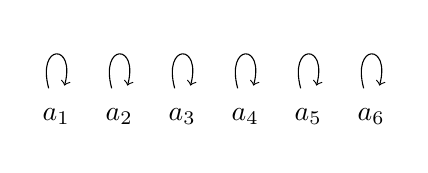
\begin{tikzpicture}
      [scale=.8,auto=left,every node/.style={circle}]

      \foreach \el/\x/\val in {n1/1/a_1, n2/2/a_2, n3/3/a_3, n4/4/a_4, n5/5/a_5, n6/6/a_6}
        \node (\el) at (\x, 0) {$\val$};

      \foreach \el/\x/\val in {n1/1/a_1, n2/2/a_2, n3/3/a_3, n4/4/a_4, n5/5/a_5, n6/6/a_6}
        \path (\el) edge [anchor=center,loop above] node {} (\el);

    \end{tikzpicture}
  \end{center}
\end{figure}

When analysing data flow graphs, such as the one above, any partitioning that doesn't sever edges denotes a valid parallel strategy. Since Figure~\ref{fig:mapgraph} contains no inter-node dependencies, it is trivial to schedule the task concurrently on many compute units.

\algblockdefx[Pf]{PFor}{EndPFor}{\textbf{in parallel, for} }{\textbf{end parallel for}}
\begin{algorithm}
  \caption{\emph{Map} higher-order function with parallel execution.}
  \label{alg:parmap}

  \begin{algorithmic}
    \Function{ParMap}{$f, A$}
      \PFor{$a_i \in A$}
        \State{$a_i \Leftarrow$ \Call{$f$}{$a_i$}}
      \EndPFor
    \EndFunction
  \end{algorithmic}
\end{algorithm}

\paragraph*{Equivalent \ac{OpenCL} kernel design}
The \ac{OpenCL} execution model suggests performing tasks over a dataset by scheduling many distinct work-units. As a result, the side-effects of Algorithm~\ref{alg:parmap}'s loop body are now provided by the result of many individual kernel-function invocations. Algorithm~\ref{alg:oclmap} describes an \ac{OpenCL} kernel that performs \verb|map| computation with a size $\|A\|$ work-group.

\begin{algorithm}
  \caption{\emph{Map} higher-order function in OpenCL kernel form.}
  \label{alg:oclmap}

  \begin{algorithmic}
    \State{$f \Leftarrow$ \Call{MutationFunction}{}}

    \Function{MapKernel}{$A$}
      \State{\Call{DeclareVariables}{$f$}}
      \State{$i \Leftarrow$ \Call{GetGlobalID}{}}
      \State{$a_i \Leftarrow$ \Call{$f$}{$a_i$}}
    \EndFunction
  \end{algorithmic}
\end{algorithm}

\paragraph*{Alternative kernel investigation}
\subparagraph*{Motivation}
After producing a system that performs \verb|map| parallelisation akin to Algorithm~\ref{alg:oclmap}, suspicion arose over whether it was excessive to schedule one work-unit per element. With traditional threaded programming, there is a significant performance cost when creating each parallel subroutine. In addition, with many kernel invocations all writing to offsets in the globally-available $A$, it was theorised that large numbers of competing memory access requests would hamper throughput.

\subparagraph*{Kernel adaption}
In order to ensure that any anticipated scaling issues were avoided, a new kernel design was constructed. The alternate design avoids scheduling a number of work-units greater than the number of compute-units present.

\begin{algorithm}
  \caption{\emph{Map} higher-order function in reduced-work-unit OpenCL kernel form.}
  \label{alg:oclmap2}

  \begin{algorithmic}
    \State{$f \Leftarrow$ \Call{MutationFunction}{}}
    \State{$width \Leftarrow \ceil{\frac{\|A\|}{compute\_units}}$}


    \Function{MapKernel}{$A, width, \|A\|$}
      \State{\Call{DeclareVariables}{$f$}}
      \State{$i \Leftarrow$ \Call{GetGlobalID}{}}
      \State{$i_{initial} \Leftarrow i \times width$}
      \State{$i_{next} \Leftarrow (i + 1) \times width$}
      \For{$i \in ((i_{initial} \ldots (i_{next} - 1) \cap (i_{initial} \ldots (\|A\| - 1))$}
        \State{$a_i \Leftarrow$ \Call{$f$}{$a_i$}}
      \EndFor
    \EndFunction
  \end{algorithmic}
\end{algorithm}

The adapted kernel, now performing \verb|map| computation using a size $\|CU\|$ work-group, is presented in Algorithm~\ref{alg:oclmap2}.

\subparagraph*{Results}
After benchmarking the execution time of the kernels presented in Algorithms \ref{alg:oclmap} and \ref{alg:oclmap2}, no significant difference in performance was found. This suggests that the overhead for work-unit scheduling within the \ac{OpenCL} framework is very low. It also suggests that simultaneous access to neighbouring global-buffer elements does not affect latency worse than strided simultaneous access.

Influenced by these findings, the decision was made to use Algorithm~\ref{alg:oclmap} for \verb|map| tasks. This is due to the design being conceptually simpler, and therefore choosing the most basic solution that works well.
\todo{Verify this conclusion on desktop}

\subsection{Scan}
\verb|Reduce| is a higher-order function that takes an array and an initial `result' value (usually an identity value) and then repeatedly applies a combining function to produce an output.

The final result is equivalent to repeatedly updating the initial value with the output of itself and the next set member using the combiner. Using this technique, the input array is consumed once while the result is cumulatively generated. Any associative reduction function can be parallelised to increase throughput.

A well-known example of reduction is when the initial value is $0$ and the combining function is \verb|+(x, y)|. This results in \emph{summation} of an input dataset.

\verb|Scan| is similar to \verb|Reduce| in that it takes an input vector and a combining function.

Instead of returning the final result, Scan returns a vector that is equal to the intermediate values if the combining function was incrementally applied from one end of the dataset to the other. \verb|Scan| can also exploit a highly-parallel architecture when supplied with suitable operators.

\paragraph*{Algorithm design}
\begin{algorithm}
  \caption{\emph{Inclusive Scan} higher-order function with sequential execution.}
  \label{alg:seqscan}

  \begin{algorithmic}
    \Function{SeqScan}{$f, a_{-1}, A$}
      \ForAll{$a_i \in A$}
      \State{$a_i \Leftarrow$ \Call{$f$}{$a_{i-1} , a_i$}}
      \EndFor
    \EndFunction
  \end{algorithmic}
\end{algorithm}

Unlike sequential \verb|map|, iteration $i$ now reads from both $a_{i-1}$ and $a_{i}$ in addition to writing $a_i$. This produces a data-dependency graph with greater connectedness, shown in Figure~\ref{fig:scangraph}

\todo{stop flipping between dependency and flow}

\begin{figure}[h]
  \caption{\emph{Inclusive Scan} dependency graph}
  \label{fig:scangraph}
  \begin{center}
    \begin{tikzpicture}
      [scale=.8,auto=left,every node/.style={circle}]

      \node (init) at (0, 0) {$initial$};
      \foreach \el/\x/\val in {n1/1/a_1, n2/2/a_2, n3/3/a_3, n4/4/a_4, n5/5/a_5, n6/6/a_6}
        \node (\el) at (2 * \x, 0) {$\val$};


      \foreach \el/\prev in {n1/init, n2/n1, n3/n2, n4/n3, n5/n4, n6/n5} {
        \path (\el) edge [anchor=center,loop above] node {} (\el);
        \draw[->] (\el) -- (\prev);
      }

    \end{tikzpicture}
  \end{center}
\end{figure}


\subsection{Filter}
